\subsection{Phonological objects in \CVCV}
\label{subsec:intro:obj}

This section briefly introduces the representation
of different phonological objects in the language of
\CVCV.

\TODO{Reihenfolge}

\TODO{vllt alles eine Hierarchieebene höher $\implies$ flache Hierarchie?}

\subsubsection{Long vowels}
Long vowels span two Nuclei, one of which is the \emph{head}
while the other needs to be licensed. Whether the first or the
second Nucleus acts as the head is a language-dependent parameter.

\begin{figure}[h]
  \centering
  \begin{subfigure}{.49\textwidth}
    \centering
    \begin{structure}{}
      \drawCV{1}
      \C{C}
      \V{V}
      \emptyC
      \emptyV
      \draw[dashed] (pV1) -- (V2);
      \draw[<-] (V2.north) -- ++(0,0.2) -- node[above]{Lic} ++(1,0);
    \end{structure}
    \caption{head-initial long vowels}    
    \label{fig:intro:longV:left-headed}
  \end{subfigure}
  \hfill
  \begin{subfigure}{.49\textwidth}
    \centering
    \begin{structure}{}
      \drawCV{1}
      \C{C}
      \longV{V}
    \end{structure}
    \caption{head-final long vowels}
    \label{fig:intro:longV:right-headed}
  \end{subfigure}
  \caption{2 kinds of long vowels}
  \label{fig:intro:longV}
  % \captionsource{long vowel headedness}{\cite[p.~267]{scheer2004}}
\end{figure}

Since government and licensing are strictly directional
(both regressive), a left-headed long vowel needs external
licensing support for its complement
(\cref{fig:intro:longV:left-headed}).
Phenomena like \tr{vowel length alternations} are \tr{zurückführen auf} this \tr{dependance}
on an external licensor.

Head-final long vowels on the other hand are self-sufficient,
their head licenses its complement (\cref{fig:intro:longV:right-headed})
and they are predicted to be \tr{unbeeinflusst vom Kontext}.


\subsubsection{Coda}\label{intro:obj:coda}
Coda consonants are defined as Onsets that occur before
a governed empty Nucleus. \parencite[p.~192]{scheer2004}
This Nucleus can either be governed by a following full
vowel, \wordunsure{IG} or because it is the final
vowel in the domain.
\Cref{fig:intro:obj:coda} shows the two different kinds
of Codas.
\marknote{2 kinds, but with IG 3 options were mentioned before?!}

\begin{figure}[h]
  \centering
  \begin{subfigure}{.49\textwidth}
    \centering
    \begin{structure}{}
      \drawCV{2}
      \V{V}
      \C{C}
      \C{\bfseries C}
      \emptyV[gov]
      \C{C}
      \V{V}
    \end{structure}
    \caption{internal Coda}
  \end{subfigure}
  \hfill
  \begin{subfigure}{.49\textwidth}
    \centering
    \begin{structure}{}
      \drawCV{1}
      \V{V}
      \C{C}
      \C{\bfseries C}
      \fen
    \end{structure}
    \caption{final Coda}
  \end{subfigure}
  \caption{Codas in \CVCV}
  \label{fig:intro:obj:coda}
\end{figure}
\TODO{hier schon positional strength of Coda/Coda-Mirror einführen?}

\begin{figure}
  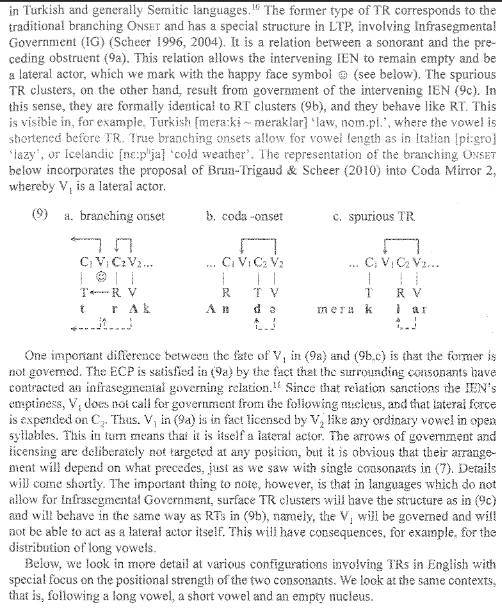
\includegraphics{figures/note_phon_objects_coda_ig.png}
  \caption{from \cite[p.~12]{scheerCyran2017}}
\end{figure}


\subsubsection{Margin contexts:}
\subsubsection{Word-start \ctx{\#\_}}\label{intro:obj:word start}
\begin{structure}{}
  \drawCV{0}
  \wordstart

  \C{C}
  \V{V}
\end{structure}
\TODO{}

\subsubsection{Syllabic consonants}
\TODO{}

\subsubsection{Branching Onsets (Infrasegmental Government)}
\TODO{}

\subsubsection{Vowel-Zero-Alternations}
\TODO{}

\begin{itemize}\color{red}
  \item Havlík: every other alternation site is vocalised,
    counting from the right edge of the sequence\par
    \q[p.~508]{scheer2004}{They may be informally stated as under (306) below.
    \begin{itemize}[widest=(306), leftmargin=*]
    \item[(306)] the two patterns of vowel-zero alternations
      \begin{enumerate}[label=\alph*.]
        \item Havlík\\
          given a chain of alternation sites, vocalise every other one,
          counting from the right margin.
        \item Lower\\
          given a chain of alternation sites, vocalise all of them
          save the last one.
      \end{enumerate}
    \end{itemize}}
\end{itemize}